\documentclass[11pt,a4paper]{article}
\usepackage[margin=2.5cm]{geometry}
\usepackage{amsmath,amssymb,bm,mathtools}
\usepackage{booktabs}
\usepackage{graphicx}
\usepackage[dvipsnames]{xcolor}
\usepackage[colorlinks=true,linkcolor=blue!50!black,citecolor=blue!50!black,urlcolor=blue!50!black]{hyperref}
\usepackage{caption}
\usepackage{enumitem}
\captionsetup{font=small,labelfont=bf}
\emergencystretch=1.5em

\newcommand{\kT}{k_{\mathrm B}T}
\newcommand{\dd}{\mathrm{d}}
\newcommand{\avg}[1]{\left\langle #1\right\rangle}
\newcommand{\lam}{\bm{\lambda}}
\newcommand{\Wd}{W_{\rm diss}}
\newcommand{\dFJ}{\widehat{\Delta F}_J}

\title{\textbf{Nonequilibrium free energies of a pulled polymer:\\
Jarzynski, Crooks, and the cost of chain length}}
\author{Youssef Kabbaj\\[0.2em]\small EPFL, Lausanne}
\date{October 2026}

\begin{document}
\maketitle

\begin{abstract}
The Jarzynski equality and the Crooks fluctuation theorem relate the work performed in arbitrarily
fast, irreversible processes to equilibrium free-energy differences. They are exact, but the
exponential averages they involve are dominated by rare trajectories, which limits their practical
use. We study this limitation in a minimal model where every quantity can be checked against an exact
answer: a two-dimensional bead--spring chain, anchored at one end and stretched by a harmonic trap
moving through a Langevin heat bath. Exact equilibrium sampling and a numerically exact free-energy
reference allow us to separate the physics from the statistics. With $10^5$ pulls per condition we find
that the dissipated work, measured in units of $\kT$, is controlled by a single combination
$\beta\Wd\simeq(\pi^2/6)\,N/(\tau/\tau_1)$ of the chain length $N$ and the pulling time $\tau$ relative to
the slowest relaxation time $\tau_1$. At fixed reduced speed it is independent of temperature, and the
work distributions at different temperatures collapse. It grows linearly with $N$, so the number of
pulls needed by the Jarzynski estimator grows exponentially with chain length. At $N=40$ the one-sided
estimate is off by $1.5\,\kT$ even with $10^5$ pulls, while Bennett's acceptance ratio, which combines
forward and reverse pulls, recovers the exact free energy to within $0.01\,\kT$. Plotting the
distribution of the Jarzynski weight $e^{-\beta W}$ shows directly why: the exponential average is
carried by trajectories that are typical of the \emph{reverse} process and are essentially never
sampled in the forward one.
\end{abstract}

%=====================================================================
\section{Introduction}

Free-energy differences determine equilibrium constants, binding affinities and the mechanical
stability of molecules. Classically they are measured along reversible, quasi-static paths, on which the
work equals the free-energy change. Jarzynski showed in 1997 that this restriction is unnecessary: for a
system that starts in equilibrium and is driven by an external parameter along \emph{any} protocol,
\begin{equation}
\avg{e^{-\beta W}}=e^{-\beta\Delta F},
\label{eq:JE}
\end{equation}
where $W$ is the work done in one realisation, $\beta=1/\kT$, and the average runs over repetitions of
the process \cite{J97}. Crooks later derived the stronger statement that forward and time-reversed work
distributions are related by $P_F(W)/P_R(-W)=e^{\beta(W-\Delta F)}$ \cite{C99}. Both relations have been
verified in single-molecule pulling experiments on RNA hairpins \cite{L02,C05} and are now standard tools
in stochastic thermodynamics \cite{Seifert}.

Their practical limitation is statistical. The average in \eqref{eq:JE} is dominated by rare
realisations in which the work falls \emph{below} $\Delta F$. Such realisations are exponentially rare
in the dissipated work $\Wd=\avg W-\Delta F$, so the number of repetitions needed grows like
$e^{\beta\Wd}$ \cite{J06,G03}. Since dissipation is generally extensive, this suggests an exponential cost
in system size. That cost is the usual reason given for why these relations are tools for single molecules rather than for macroscopic
systems.

In this work we make these statements quantitative in a model simple enough to be solved exactly at
equilibrium, yet rich enough to have non-trivial, entropic elasticity: a two-dimensional chain of $N$
beads, anchored at one end and stretched by a moving optical-tweezer-like trap. The model has three
properties that are rarely available together. Its equilibrium free energy can be computed exactly for
any $N$ and $T$. Its initial equilibrium ensemble can be sampled exactly, without equilibration runs.
And a Gaussian limit of the model gives the full work distribution of the discretised dynamics in
closed form. Every estimate below can therefore be compared with the truth, and simulation errors can
be separated from estimator errors.

Our main findings are the following. (i) A simple affine-stretching argument predicts the dissipated work
to within about $12\%$ for $N\ge10$. In units of $\kT$ it depends only on $N$ and on the pulling time
in units of the chain's relaxation time. (ii) As a consequence, the work distributions of an entropic
chain at different temperatures collapse onto one curve when the pulling time is scaled with the relaxation time.
(iii) The one-sided Jarzynski estimator fails exponentially in chain length, and its bootstrap error bars
are over-confident by a factor of about three. (iv) The Crooks theorem holds with log-ratio slopes within
$2\%$ of the predicted value. The two-sided Bennett estimator recovers $\Delta F$ to $0.01\,\kT$ precisely where the one-sided estimators fail. (v) Visualising the
distribution of $e^{-\beta W}$ explains (iii) and (iv) directly through the Crooks identity.

%=====================================================================
\section{Model and methods}

Derivations are given in a companion theory document \cite{theory}; here we state what is needed to
follow the results.

\subsection{Anchored chain in a moving trap}

The chain consists of beads $\bm r_0,\dots,\bm r_N\in\mathbb R^2$ of mass $m$. Bead $0$ is fixed at the
origin, and bead $N$ is held by a harmonic trap of stiffness $k_t$ centred at $\lam$:
\begin{equation}
H(\bm x;\lam)=\sum_{i=1}^N\frac{|\bm p_i|^2}{2m}+\sum_{i=1}^N\frac{k}{2}\big(|\bm r_i-\bm r_{i-1}|-b\big)^2
+\frac{k_t}{2}|\bm r_N-\lam|^2 .
\end{equation}
We consider two versions. For $b=0$ (Gaussian or Rouse chain) all forces are linear and the elasticity
is energetic. For $b=1$ with stiff bonds ($k=100$, so bond-length fluctuations are $\sim10\%$ at $\kT=1$)
the chain is nearly freely jointed and its elasticity is entropic. The chain is a phantom chain:
non-bonded beads do not interact. The trap moves at constant speed along $x$,
$\lam(t)=(x_0+(x_1-x_0)t/\tau,0)$, from $x_0=0.2L$ to $x_1=0.7L$, where $L=Nb$ is the contour length
($L=0.3N$ for $b=0$). Units are $m=b=\varepsilon=1$; we use $k_t=10$ and friction rate $\gamma=1$
throughout.

\subsection{Dynamics, work and fluctuation theorems}

Each mobile bead follows underdamped Langevin dynamics,
$\dd\bm p_i=-\nabla_iH\,\dd t-\gamma\bm p_i\,\dd t+\sqrt{2\gamma m\kT}\,\dd\bm B_i$. The friction and noise
model collisions with the solvent; their strengths are tied by the fluctuation--dissipation relation,
which makes the canonical distribution $\rho_{\rm eq}\propto e^{-\beta H}$ stationary at every fixed $\lam$.
The work done by the moving trap in one pull is
\begin{equation}
W=\int_0^\tau\frac{\partial H}{\partial\lam}\cdot\dot\lam\,\dd t=-k_t\int_0^\tau(\bm r_N-\lam)\cdot\dot\lam\,\dd t .
\end{equation}
Equation \eqref{eq:JE} holds whenever the chain starts in equilibrium and the dynamics at frozen $\lam$
preserves the canonical distribution. The Crooks theorem additionally involves the reverse protocol
($x_1\to x_0$ in the same time, starting in equilibrium at $x_1$). It implies
\begin{equation}
\frac{e^{-\beta W}P_F(W)}{\avg{e^{-\beta W}}_F}=P_R(-W),
\label{eq:share}
\end{equation}
which we use repeatedly. The share of the exponential average contributed by forward works near $W$
equals the mirrored reverse work distribution.

We compare three estimators of $\Delta F$:
\begin{itemize}[leftmargin=*,itemsep=1pt]
\item the forward Jarzynski estimator $\dFJ=-\kT\ln\big(M^{-1}\sum_me^{-\beta W_m}\big)$;
\item its reverse counterpart $+\kT\ln\big(M^{-1}\sum_me^{-\beta W^R_m}\big)$;
\item Bennett's acceptance ratio (BAR), the root of
$\sum_F\mathrm f(\beta(W_m-\Delta F))=\sum_R\mathrm f(\beta(W^R_m+\Delta F))$ with $\mathrm f(x)=1/(1+e^x)$ for
equal sample sizes. BAR is the minimum-variance and maximum-likelihood combination of both directions \cite{B76,S03}.
\end{itemize}
As diagnostics we report the effective sample size $M_{\rm eff}=(\sum w_m)^2/\sum w_m^2$ of the weights
$w_m=e^{-\beta W_m}$ and the convergence of $\dFJ$ with the number of pulls used.

\subsection{Exact reference free energies}

In bond variables $\bm u_i=\bm r_i-\bm r_{i-1}$ the bonds are independent except for the trap, so the
partition function is a convolution, $Z(\lam)\propto(g^{*N}*w)(\lam)$, of the bond Boltzmann factor $g$
with itself $N$ times and with the trap factor $w$. For $b=0$ this gives
$\Delta F=\tfrac12k_{\rm eff}(x_1^2-x_0^2)$ with $1/k_{\rm eff}=N/k+1/k_t$, independent of temperature. For
$b=1$ we evaluate the radial two-dimensional convolutions numerically in log space. The equivalent
Fourier-space formula loses all precision through cancellation once $\beta\Delta F\gtrsim10$. The
log-space method reproduces the closed form to $10^{-4}$. Table~\ref{tab:dF} lists the values used. For the
entropic chain $\Delta F/\kT$ is nearly temperature independent, as expected for rubber elasticity. The
Gaussian ``entropic-spring'' approximation misses up to $12\%$ (finite extensibility at $N=40$) and even
has the wrong sign of error for $N=5$, where a short two-dimensional chain is strongly non-Gaussian.

\begin{table}[t]
\centering\small
\begin{tabular}{lccccccc}
\toprule
& $N=5$ & $N=10$ & $N=20$ & $N=40$ & & $\kT=0.25$ & $\kT=2$\\
\midrule
exact $\beta\Delta F$ & $1.98$ & $4.42$ & $9.49$ & $19.69$ & & $4.62$ & $4.18$\\
entropic spring & $2.10$ & $4.29$ & $8.65$ & $17.39$ & & $4.44$ & $4.09$\\
\bottomrule
\end{tabular}
\caption{Free-energy differences of the stiff-bond chain for the protocol $0.2L\to0.7L$ (left: $\kT=1$; right: $N=10$),
in units of $\kT$.}
\label{tab:dF}
\end{table}

\subsection{Simulation}

\paragraph{Integrator.} The Langevin equations are integrated with the BAOAB splitting \cite{LM13},
$\Delta t=0.01$. The trap position is updated in discrete steps, and the work is accumulated as the energy
jump $H(\bm x;\lam_{k+1})-H(\bm x;\lam_k)$ at fixed configuration before each integrator step. This
switch-then-relax construction satisfies a discrete-time version of \eqref{eq:JE}, up to the
$O(\Delta t^2)$ error with which a BAOAB step preserves the canonical distribution. For the Gaussian
chain, propagating means and covariances through the linear update rules gives the exact work statistics
of the discrete algorithm. The residual violation of \eqref{eq:JE} is $8\times10^{-4}\,\kT$ and scales as
$\Delta t^2$. Halving $\Delta t$ for the stiff chain changes no estimate beyond its statistical scatter
(Appendix~\ref{app:checks}).

\paragraph{Exact initial states.} Pulls must start in equilibrium. Instead of equilibrating each chain
dynamically, we draw exact samples by rejection. Chains are proposed with independent bonds that feel a
constant pulling force $f$, and each is accepted with probability $e^{-\beta k_t|\bm R-\lam'|^2/2}$, where
$\bm R$ is the end-to-end vector and $\lam'=\lam-(f/k_t)\hat{\bm x}$. The procedure is exact for any $f$.
Choosing $f$ equal to the chain tension at the target extension raises the acceptance rate from
$\sim10^{-9}$ to $\sim1\%$ for the most stretched states ($N=40$ at $0.7L$).

\paragraph{Relaxation time and protocols.} Pulling times are measured in units of $\tau_1=\zeta/\lambda_{\min}(K)$,
the slowest relaxation time of the linearised (Rouse) chain. Here $\zeta=m\gamma$ and $K$ is the stiffness matrix of a chain of
entropic springs $\kappa=2\kT/\avg{u^2}$ with the stiff trap at its end. Because the trap nearly clamps the end,
$\tau_1\simeq\zeta N^2\avg{u^2}/2\pi^2\kT$, giving $\tau_1=1.45,5.46,21.3,84.3$ for $N=5,10,20,40$ at $\kT=1$.
In a slow pull the chain stretches affinely, with bead $i$ moving at speed $v\,i/N$. The friction power is then
$\zeta Nv^2/3$, which yields the estimate
\begin{equation}
\beta\Wd\simeq\frac{\zeta N(x_1-x_0)^2}{3\kT\tau}=\frac{\pi^2}{6}\,\frac{N}{\tau/\tau_1}.
\label{eq:affine}
\end{equation}

\paragraph{Statistics.} Each condition uses $M=10^5$ independent pulls, integrated in parallel on a GPU.
All code is covered by unit tests, which check forces, exact sampling, the exact Gaussian-chain moments and
Crooks relations, the first law per trajectory, and the estimators on synthetic data.

%=====================================================================
\section{Results}

\subsection{Validation on the Gaussian chain}

\begin{figure}[t]
\centering
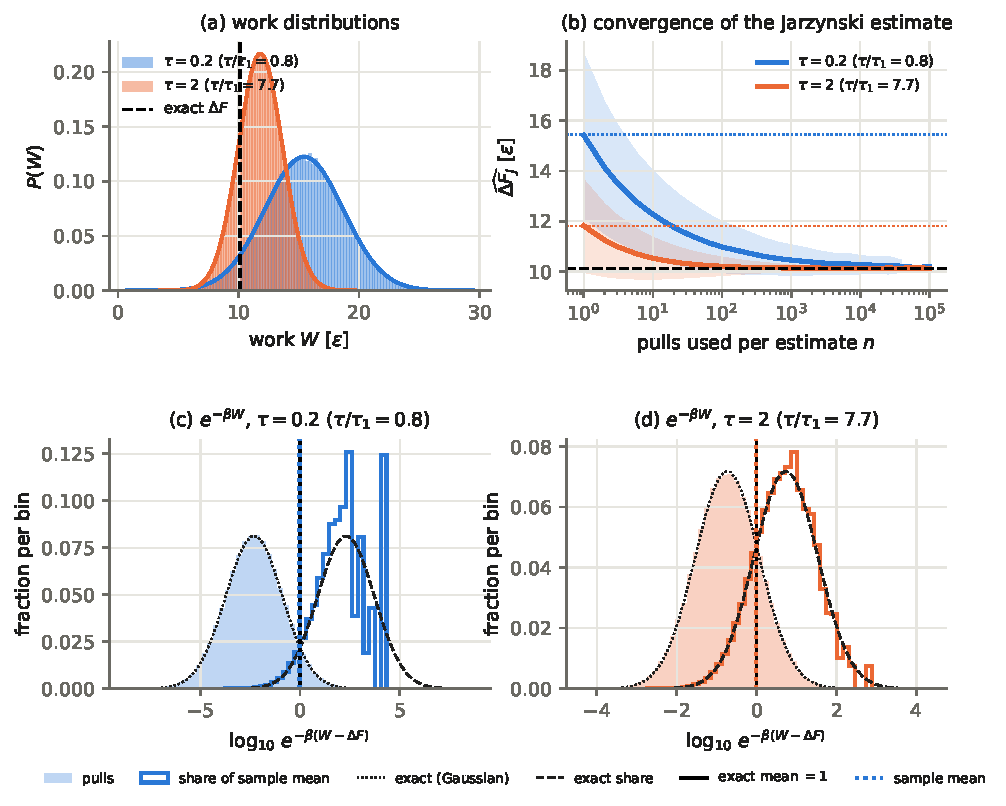
\includegraphics[width=0.92\linewidth]{../figures/F1_validation.pdf}
\caption{Gaussian chain ($b=0$, $N=10$, $\kT=1$, $\Delta F=10.125$). (a) Work distributions for a fast
($\tau=0.8\tau_1$) and a slow ($\tau=7.7\tau_1$) pull; lines are the exact distributions of the discrete
algorithm. (b) Jarzynski estimate using $n$ pulls (mean and spread over disjoint blocks); dotted lines mark
$\avg W$. (c, d) Distribution of the normalised Jarzynski weight $x=e^{-\beta(W-\Delta F)}$ (exact mean
$1$): filled, fraction of pulls; solid, share of the sample mean; dashed, exact share.}
\label{fig:F1}
\end{figure}

For the Gaussian chain the simulated mean and variance of $W$ agree with the exact values of the
discrete algorithm to $0.1\%$ and $1\%$, and the whole distributions coincide (Fig.~\ref{fig:F1}a). With
$10^5$ pulls, the Jarzynski estimator gives $10.134\pm0.015$ for the slow pull and $10.19\pm0.14$ for the
fast one ($\Delta F=10.125$), although the mean work exceeds $\Delta F$ by $1.7$ and $5.3\,\kT$. The
convergence curves (Fig.~\ref{fig:F1}b) show the characteristic behaviour: with few pulls the estimate
sits near $\avg W$, and it approaches $\Delta F$ only once rare low-work pulls have been sampled. That takes
about $100$ times more pulls for the faster protocol.

The lower panels show why. The weight $x=e^{-\beta(W-\Delta F)}$ has mean exactly one, but for Gaussian work
the pulls and the contributions to the mean are displaced from each other by $\beta^2\sigma_W^2$ in $\ln x$.
That is $1.5$ decades for the slow pull, where the sampled contributions reproduce the exact ones, and
$4.6$ decades for the fast pull. In the fast case the true mean is dominated by values of $x$ around
$10^{2.3}$, reached by only $0.06\%$ of the pulls. The sampled contributions reduce to a handful of spikes.

\subsection{Pulling speed: dissipation and where the average comes from}

\begin{figure}[t]
\centering
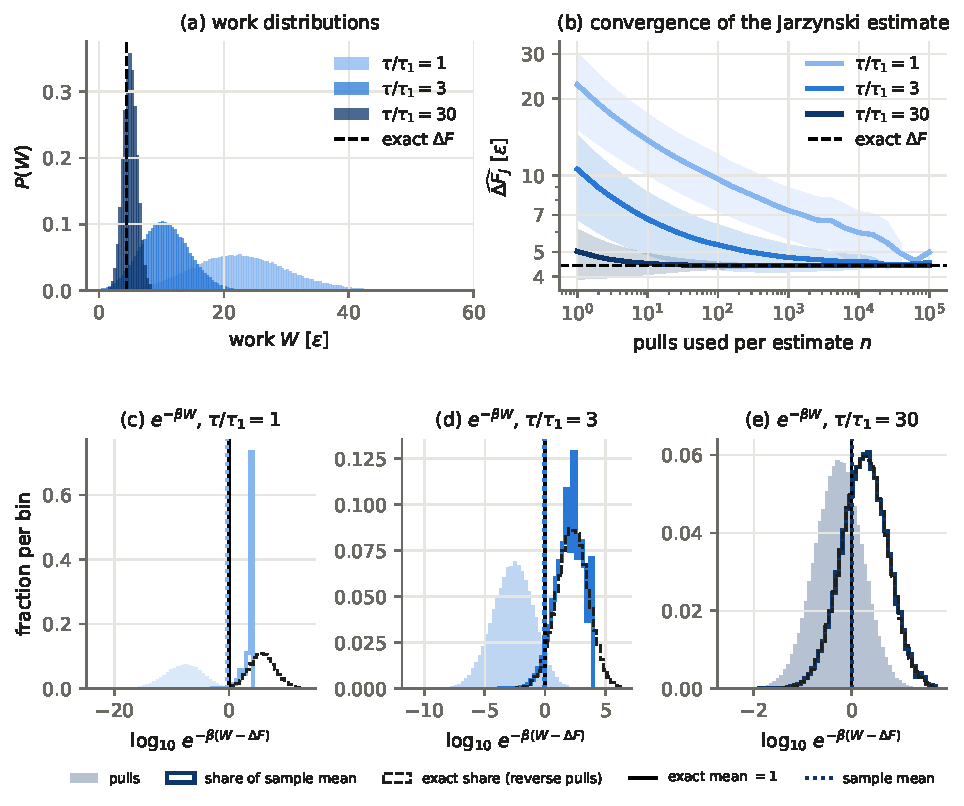
\includegraphics[width=0.92\linewidth]{../figures/F2_speed.pdf}
\caption{Stiff-bond chain ($b=1$, $N=10$, $\kT=1$, $\Delta F=4.420$, $\tau_1=5.46$) pulled at three speeds.
(a) Work distributions. (b) Convergence of the Jarzynski estimate. (c--e) Distribution of $x=e^{-\beta(W-\Delta F)}$
as in Fig.~\ref{fig:F1}; the exact share of the mean is obtained from $10^5$ reverse pulls through
Eq.~\eqref{eq:share}.}
\label{fig:F2}
\end{figure}

For the entropic chain, the dissipated work at $\tau/\tau_1=1,3,30$ is $\beta\Wd=18.3$, $6.2$ and $0.61$. The
affine estimate \eqref{eq:affine} gives $16.4$, $5.5$ and $0.55$: it is low by a constant $11$--$12\%$, so
the $1/\tau$ scaling holds down to $\tau=\tau_1$. The near-equilibrium relation $\sigma_W^2=2\kT\Wd$ holds
to $3\%$ for the slowest pull but is exceeded by factors $1.2$ and $1.5$ for the faster ones, where the
distribution also acquires a positive skew. As a result the second-cumulant estimate
$\avg W-\beta\sigma_W^2/2$, exact for Gaussian work, fails by $10\,\kT$ at $\tau=\tau_1$.

The Jarzynski estimator converges for $\tau=30\tau_1$ ($4.415\pm0.005$) and, with $10^5$ pulls, for $3\tau_1$
($4.55\pm0.10$), but not for $\tau=\tau_1$. Panels (c--e) make the reason visible, using the reverse pulls
to obtain the \emph{exact} distribution of contributions to $\avg{e^{-\beta W}}$ without any rare-event
sampling. At $\tau=\tau_1$ half of the true average comes from weights $x>10^{5.9}$, while the largest weight
among all $10^5$ forward pulls is $10^{4.3}$: no forward pull reaches the region that matters. The sample
mean is $0.57$ of the true mean and is carried by three pulls ($33\%$, $27\%$ and $14\%$ of it). The resulting
estimate, $4.99$, still looks reasonable, because the logarithm compresses the error: missing half of the
average costs only $\kT\ln2$. Nothing in the forward data alone signals the problem.

\subsection{Temperature: entropic elasticity and data collapse}

\begin{figure}[t]
\centering
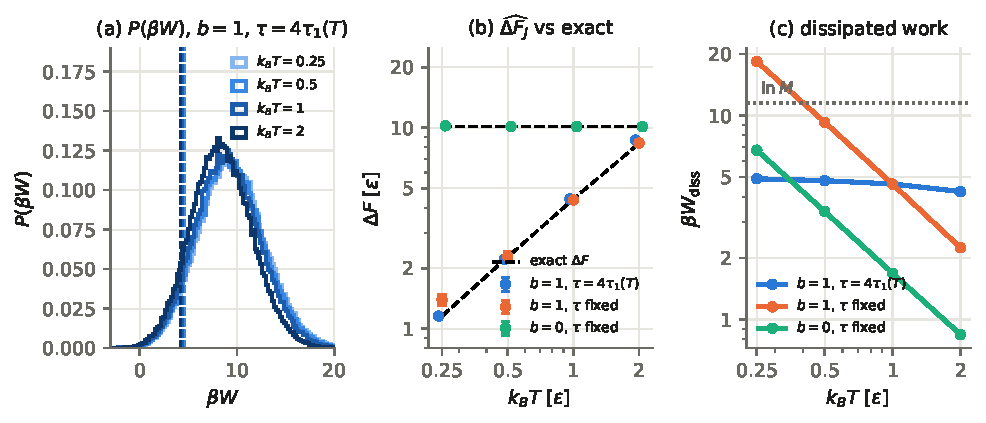
\includegraphics[width=0.92\linewidth]{../figures/F3_temperature.pdf}
\caption{Temperature dependence ($N=10$). (a) Distributions of $\beta W$ for the stiff-bond chain at fixed reduced
speed $\tau=4\tau_1(T)$; dashed lines mark $\beta\Delta F$. (b) Jarzynski estimates against the exact $\Delta F$
(dashed) for the stiff-bond chain at fixed $\tau/\tau_1$ and at fixed $\tau$, and for the Gaussian chain.
(c) Dissipated work in units of $\kT$; dotted line: $\ln M$.}
\label{fig:F3}
\end{figure}

The two chains respond to temperature in opposite ways (Fig.~\ref{fig:F3}b). For the Gaussian chain $\Delta F$
is temperature independent, as is the mean work, because the mean response of a linear system is
deterministic. The bath only broadens the distribution, $\sigma_W^2\propto T$, so $\beta\Wd\propto1/T$. For
the entropic chain $\Delta F\propto T$: a hotter chain is harder to stretch.

When the pulling time is scaled with the temperature-dependent relaxation time, $\tau=4\tau_1(T)$, the
distributions of $\beta W$ at four temperatures spanning a factor of eight fall on top of each other
(Fig.~\ref{fig:F3}a), and $\beta\Wd$ stays between $4.2$ and $4.9$. This follows from Eq.~\eqref{eq:affine}.
Both $\Delta F$ and $\Wd$ are proportional to $T$ at fixed $\tau/\tau_1$, so temperature merely changes the energy
unit. The residual drift comes from the slight thermal stretching of the bonds. At a fixed pulling
\emph{time}, by contrast, the dissipated work is set by friction and speed and is nearly temperature
independent, so $\beta\Wd\propto1/T$ ($18.4$, $9.3$, $4.6$, $2.2$). At $\kT=0.25$ it exceeds $\ln M$ and the
estimate is $20\%$ too high. Experiments in a cold bath are harder only because the same pulling speed is relatively faster.

\subsection{Chain length: an exponential cost}

\begin{figure}[t]
\centering
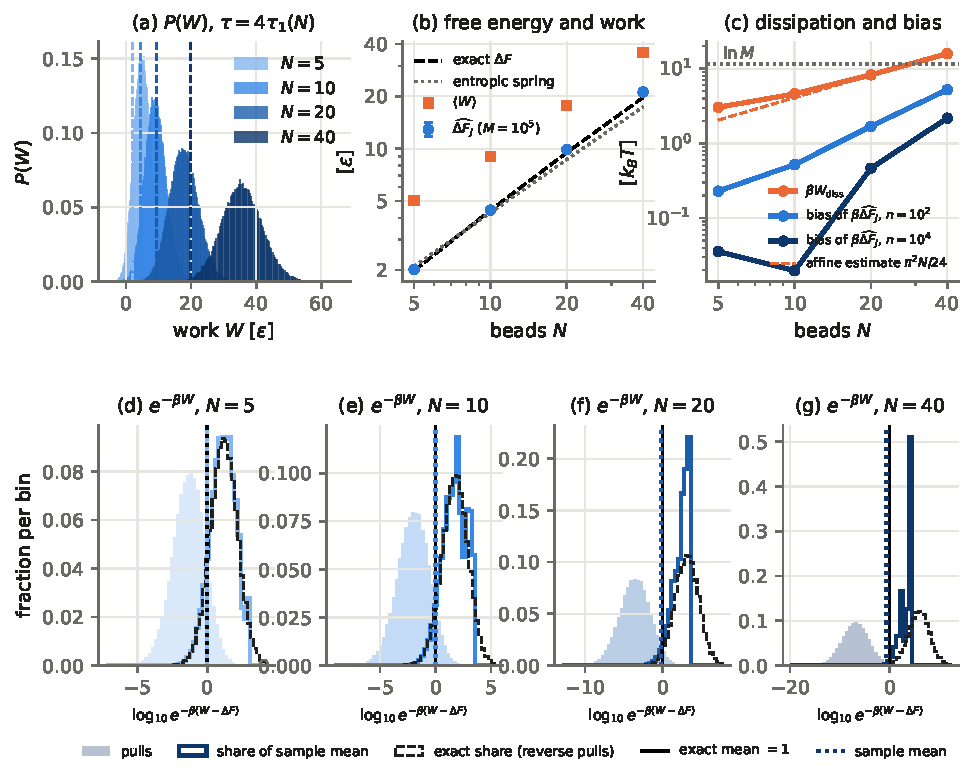
\includegraphics[width=0.92\linewidth]{../figures/F4_size.pdf}
\caption{Chain-length dependence at fixed relative extension and fixed reduced speed $\tau=4\tau_1(N)$, $\kT=1$.
(a) Work distributions. (b) Exact $\Delta F$, entropic-spring approximation, mean work and Jarzynski estimate.
(c) Dissipated work and bias of the Jarzynski estimate with $n$ pulls. (d--g) Distribution of
$x=e^{-\beta(W-\Delta F)}$ for each $N$, with the exact share from reverse pulls.}
\label{fig:F4}
\end{figure}

At fixed relative extension both $\Delta F$ and $\avg W$ are nearly extensive in $N$, while $\sigma_W$ grows
like $\sqrt N$: relative work fluctuations shrink as $1/\sqrt N$, as expected from the macroscopic
limit. At fixed reduced speed the dissipated work grows linearly, $\beta\Wd=3.1$, $4.6$, $8.3$ and $16.0$ for
$N=5$, $10$, $20$ and $40$, and approaches the affine estimate $\pi^2N/24$ (within $1\%$ at $N=20$, $3\%$ at
$N=40$). The number of pulls needed therefore grows exponentially with chain length. The Jarzynski
estimate is accurate to $0.03\,\kT$ up to $N=10$, biased by $+0.38\,\kT$ at $N=20$ and by $+1.47\,\kT$ at
$N=40$, where $M_{\rm eff}=3.6$. At fixed computational budget the bias grows steeply with $N$
(Fig.~\ref{fig:F4}c). Keeping $\beta\Wd$ fixed would require $\tau\propto N\tau_1\propto N^3$.

The lower row shows the mechanism. As $N$ grows, the pulls move to lower weights and the exact
contributions to the mean move to higher ones. At $N=40$, $81\%$ of the true average lies beyond the
largest weight observed in $10^5$ forward pulls, and a single pull carries half of the sample mean. In
the failing cases the bootstrap error bars do not cover the exact value ($3.4\sigma$ off at $N=20$, $2.7\sigma$ at
$N=40$). Where the true spread of the estimator could be measured, it was $2$--$3$ times larger than the
bootstrap estimate, because resampling the observed pulls cannot account for regions that were never
sampled (Appendix~\ref{app:checks}).

\subsection{Crooks theorem and two-sided estimation}

\begin{figure}[t]
\centering
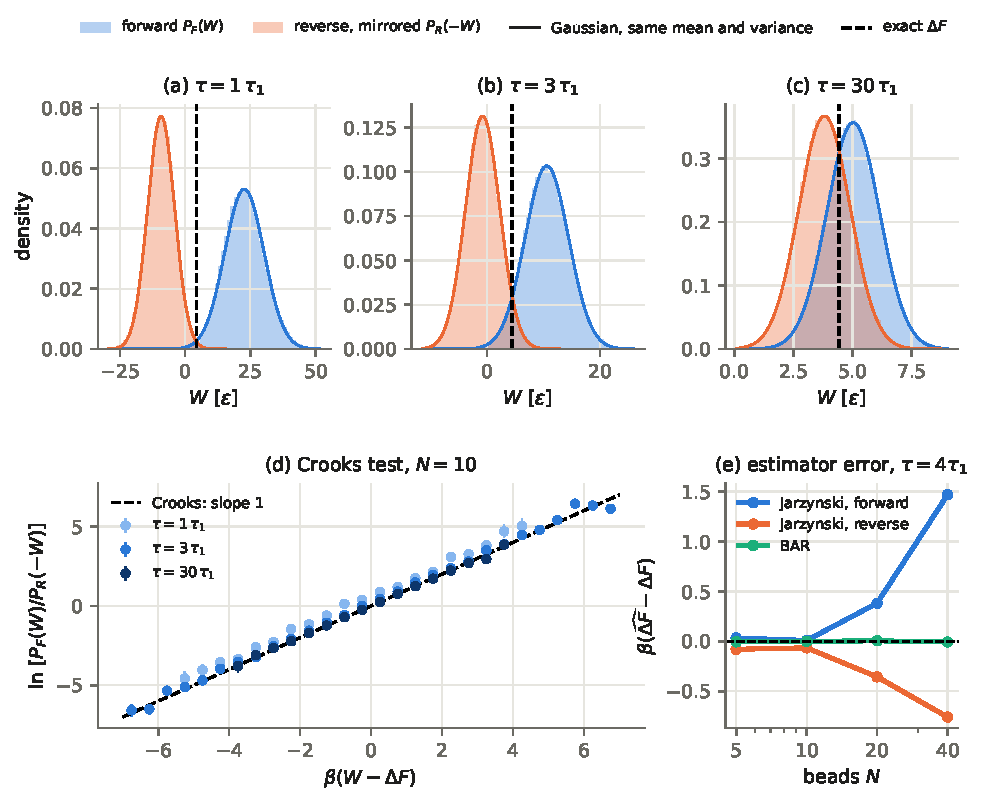
\includegraphics[width=0.92\linewidth]{../figures/F5_crooks.pdf}
\caption{Crooks theorem ($\kT=1$, $10^5$ forward and $10^5$ reverse pulls per condition). (a--c) Forward and
mirrored reverse work distributions for $N=10$ at three speeds, with Gaussians of equal mean and variance;
dashed: $\Delta F=4.420$. (d) Logarithm of their ratio against $\beta(W-\Delta F)$; the dashed line is the
prediction. (e) Error of the forward and reverse Jarzynski estimators and of BAR against chain length.}
\label{fig:F5}
\end{figure}

For every speed the forward and mirrored reverse distributions intersect at $\Delta F$
(Fig.~\ref{fig:F5}a--c), and the logarithm of their ratio is a straight line of slope $0.98$--$0.99$
(prediction: $1$), the same for all speeds (Fig.~\ref{fig:F5}d). This holds even though the distributions
change completely between $\tau=\tau_1$ and $30\tau_1$.

Forward and reverse pulls are not symmetric. The reverse pull dissipates less ($\beta\Wd^R=13.6$ against
$\beta\Wd^F=18.3$ at $\tau=\tau_1$), its distribution is narrower ($\sigma_R=5.2$ against $\sigma_F=7.5$), and
it obeys the linear-response relation $\sigma_W^2=2\kT\Wd$ within $10\%$, whereas the forward pull exceeds
it by $54\%$. Both distributions remain close to Gaussian, with skewness below $0.22$. The asymmetry
disappears near equilibrium, where Crooks forces $\Wd^F=\Wd^R$. A plausible interpretation is that a fast
forward pull drives the end of the chain into the stiff, finite-extensibility regime, where the force is
very sensitive to the chain's conformation, whereas a reverse pull releases tension towards the soft, Gaussian regime.

The asymmetry matters for estimation. By Eq.~\eqref{eq:share}, the forward estimator needs
$M\gtrsim e^{\beta\Wd^R}$ pulls to sample the region that dominates its average, and the reverse estimator
needs $e^{\beta\Wd^F}$. At $N=40$ both conditions fail with $10^5$ pulls. The one-sided estimates are off by
$+1.47$ (forward) and $-0.76\,\kT$ (reverse), in opposite directions as expected (Fig.~\ref{fig:F5}e).
BAR, which only needs the two distributions to overlap near $\Delta F$, gives $19.688\pm0.039$ against the exact
$19.694$. The overlap region contains only $0.4\%$ of the forward and $0.3\%$ of the reverse pulls, a few hundred each,
which suffices. BAR is within $0.01\,\kT$ of the exact value for all chain lengths. In the
most demanding single case ($N=10$, $\tau=\tau_1$) it is $0.08\,\kT$ low, compared with $+0.57$ and $-0.54\,\kT$ for
the one-sided estimates.

%=====================================================================
\section{Discussion}

Three points emerge that go beyond verifying the fluctuation theorems.

First, a single dimensionless number controls the practical usefulness of the Jarzynski equality in this
system: $\beta\Wd\simeq(\pi^2/6)N/(\tau/\tau_1)$. Temperature enters only through the relaxation time, and
chain length enters linearly. The exponential cost in system size, usually stated qualitatively, here takes
an explicit form. At the reduced speed used here ($\tau=4\tau_1$) the required number of pulls grows like
$e^{0.4N}$.
Doubling the chain from $20$ to $40$ beads turned a slightly biased estimate into a failed one.

Second, the standard diagnostics are unreliable exactly where they are needed. The second-cumulant
estimate fails as soon as the work distribution is skewed. The bootstrap underestimates the error because it
cannot see unsampled regions. And the Jarzynski estimate itself is deceptively stable, because the
logarithm compresses large relative errors in the exponential average. The distribution of
$e^{-\beta W}$, combined with reverse pulls through the Crooks identity, provides a direct check: if the
exact contributions to the average lie beyond the largest sampled weight, the forward estimate cannot be trusted.

Third, two-sided estimation changes the scaling of the problem. One-sided estimators need to sample the
typical region of the opposite process. BAR needs only overlap between the two, which persists much longer as
dissipation grows. In single-molecule experiments, where reverse (refolding) pulls are usually available,
this argues for collecting both directions whenever possible, as is done in practice \cite{C05}.

The model has deliberate limitations. The chain is a phantom chain without excluded volume or bending
stiffness, hydrodynamic interactions are neglected, and the motion is two-dimensional. These choices make
the exact reference possible. Adding excluded volume would require thermodynamic integration for $\Delta F$, but
should not change the qualitative picture, since the scaling argument relies only on the affine dissipation
and the extensivity of $\Wd$. The interpretation of the forward--reverse asymmetry in terms of
finite extensibility was not tested directly. Varying the bond stiffness or the extension range would test it.

Two natural extensions are protocol optimisation and feedback. Shaping $\lam(t)$, rather than only its
duration, reduces dissipation; in linear response the optimal protocol moves at constant thermodynamic
speed. No open-loop protocol can bring the mean work below $\Delta F$, but feedback protocols that react to
the measured chain can, at an information cost bounded by the Sagawa--Ueda relation.

\section{Conclusion}

We studied the Jarzynski and Crooks relations for an anchored two-dimensional chain pulled through a
Langevin bath, comparing every estimate with exact free energies obtained from a log-space convolution
and exact equilibrium sampling. The fluctuation theorems hold to within the statistical and discretisation
accuracy of the simulations. Their practical value is governed by the dissipated work, which an
affine-stretching argument predicts as $\beta\Wd\simeq(\pi^2/6)N/(\tau/\tau_1)$. This explains the collapse of
work distributions across temperatures at fixed reduced speed and the exponential growth with chain length
of the number of pulls the Jarzynski estimator requires. Plots of $e^{-\beta W}$ together with the Crooks identity
reveal when the forward estimate is missing most of its average, and Bennett's two-sided estimator recovers
the exact free energy where one-sided estimates fail by more than $\kT$.

%=====================================================================
\appendix
\section{Numerical checks}
\label{app:checks}

\paragraph{Time step.} For the Gaussian chain, the exact propagation of the discrete algorithm gives a
Jarzynski residual $\avg W-\beta\sigma_W^2/2-\Delta F=-8.0\times10^{-4}$, $-3.0\times10^{-3}$ and
$-1.1\times10^{-2}\,\kT$ at $\Delta t=0.01$, $0.02$, $0.04$, a clean $\Delta t^2$ law. The residual is non-zero
because the momentum distribution of BAOAB is slightly distorted. For the stiff chain ($N=10$, $\tau=4\tau_1$)
halving $\Delta t$ changed the three-seed mean of $\beta\dFJ$ by $-0.07$ ($\kT=2$) and $-0.05$ ($\kT=1$),
comparable to the seed-to-seed scatter, and $\avg W$ by less than $0.1\%$.

\paragraph{Error bars.} For Gaussian work the sampling distribution of $\dFJ$ can be simulated directly. At
$\beta\Wd=6.8$ and $M=10^5$ it has mean bias $+0.10\,\kT$ and spread $0.28\,\kT$, three times the bootstrap
estimate from a single sample. Independent repetitions of the stiff-chain run at $\kT=2$ scatter by $0.09\,\kT$,
twice the bootstrap error. We therefore recommend independent repetitions or block-convergence curves
rather than bootstrap errors whenever $M_{\rm eff}$ is below a few thousand.

\paragraph{Reference free energies.} The log-space convolution agrees with the closed form for $b=0$
($64.796$ against $64.800$ at $N=40$) and with the Fourier-space formula wherever the latter is numerically
reliable. The mean trap force sampled from the exact equilibrium ensemble agrees with $\partial F/\partial\lambda$
from the reference.

\begin{thebibliography}{99}
\bibitem{J97} C.~Jarzynski, Nonequilibrium equality for free energy differences, Phys.\ Rev.\ Lett.\ \textbf{78}, 2690 (1997).
\bibitem{C99} G.~E.~Crooks, Entropy production fluctuation theorem and the nonequilibrium work relation for free
energy differences, Phys.\ Rev.\ E \textbf{60}, 2721 (1999).
\bibitem{L02} J.~Liphardt, S.~Dumont, S.~B.~Smith, I.~Tinoco, C.~Bustamante, Equilibrium information from
nonequilibrium measurements in an experimental test of Jarzynski's equality, Science \textbf{296}, 1832 (2002).
\bibitem{C05} D.~Collin, F.~Ritort, C.~Jarzynski, S.~B.~Smith, I.~Tinoco, C.~Bustamante, Verification of the Crooks
fluctuation theorem and recovery of RNA folding free energies, Nature \textbf{437}, 231 (2005).
\bibitem{Seifert} U.~Seifert, Stochastic thermodynamics, fluctuation theorems and molecular machines, Rep.\ Prog.\
Phys.\ \textbf{75}, 126001 (2012).
\bibitem{J06} C.~Jarzynski, Rare events and the convergence of exponentially averaged work values, Phys.\ Rev.\ E
\textbf{73}, 046105 (2006).
\bibitem{G03} J.~Gore, F.~Ritort, C.~Bustamante, Bias and error in estimates of equilibrium free-energy differences
from nonequilibrium measurements, PNAS \textbf{100}, 12564 (2003).
\bibitem{B76} C.~H.~Bennett, Efficient estimation of free energy differences from Monte Carlo data, J.\ Comput.\
Phys.\ \textbf{22}, 245 (1976).
\bibitem{S03} M.~R.~Shirts, E.~Bair, G.~Hooker, V.~S.~Pande, Equilibrium free energies from nonequilibrium
measurements using maximum-likelihood methods, Phys.\ Rev.\ Lett.\ \textbf{91}, 140601 (2003).
\bibitem{LM13} B.~Leimkuhler, C.~Matthews, Rational construction of stochastic numerical methods for molecular
sampling, Appl.\ Math.\ Res.\ Express \textbf{2013}, 34 (2013).
\bibitem{theory} Companion theory document \texttt{theory.pdf} (model, three derivations of the Jarzynski equality,
Crooks theorem, estimator derivations, numerical scheme), in the same repository.
\end{thebibliography}

\end{document}
